% Options for packages loaded elsewhere
\PassOptionsToPackage{unicode}{hyperref}
\PassOptionsToPackage{hyphens}{url}
%
\documentclass[
  11pt,
]{article}
\usepackage{amsmath,amssymb}
\usepackage{lmodern}
\usepackage{iftex}
\ifPDFTeX
  \usepackage[T1]{fontenc}
  \usepackage[utf8]{inputenc}
  \usepackage{textcomp} % provide euro and other symbols
\else % if luatex or xetex
  \usepackage{unicode-math}
  \defaultfontfeatures{Scale=MatchLowercase}
  \defaultfontfeatures[\rmfamily]{Ligatures=TeX,Scale=1}
\fi
% Use upquote if available, for straight quotes in verbatim environments
\IfFileExists{upquote.sty}{\usepackage{upquote}}{}
\IfFileExists{microtype.sty}{% use microtype if available
  \usepackage[]{microtype}
  \UseMicrotypeSet[protrusion]{basicmath} % disable protrusion for tt fonts
}{}
\makeatletter
\@ifundefined{KOMAClassName}{% if non-KOMA class
  \IfFileExists{parskip.sty}{%
    \usepackage{parskip}
  }{% else
    \setlength{\parindent}{0pt}
    \setlength{\parskip}{6pt plus 2pt minus 1pt}}
}{% if KOMA class
  \KOMAoptions{parskip=half}}
\makeatother
\usepackage{xcolor}
\usepackage[margin=1.0in]{geometry}
\usepackage{graphicx}
\makeatletter
\def\maxwidth{\ifdim\Gin@nat@width>\linewidth\linewidth\else\Gin@nat@width\fi}
\def\maxheight{\ifdim\Gin@nat@height>\textheight\textheight\else\Gin@nat@height\fi}
\makeatother
% Scale images if necessary, so that they will not overflow the page
% margins by default, and it is still possible to overwrite the defaults
% using explicit options in \includegraphics[width, height, ...]{}
\setkeys{Gin}{width=\maxwidth,height=\maxheight,keepaspectratio}
% Set default figure placement to htbp
\makeatletter
\def\fps@figure{htbp}
\makeatother
\setlength{\emergencystretch}{3em} % prevent overfull lines
\providecommand{\tightlist}{%
  \setlength{\itemsep}{0pt}\setlength{\parskip}{0pt}}
\setcounter{secnumdepth}{5}
\newcommand{\bcenter}{\begin{center}}
\newcommand{\ecenter}{\end{center}}
\newcommand{\btitlepage}{\begin{titlepage}}
\newcommand{\etitlepage}{\end{titlepage}}
\usepackage{helvet}
\renewcommand*\familydefault{\sfdefault}
\usepackage{setspace}\doublespacing
\usepackage{booktabs}
\usepackage[font=small,labelfont=bf]{caption}
\ifLuaTeX
  \usepackage{selnolig}  % disable illegal ligatures
\fi
\IfFileExists{bookmark.sty}{\usepackage{bookmark}}{\usepackage{hyperref}}
\IfFileExists{xurl.sty}{\usepackage{xurl}}{} % add URL line breaks if available
\urlstyle{same} % disable monospaced font for URLs
\hypersetup{
  hidelinks,
  pdfcreator={LaTeX via pandoc}}

\author{}
\date{\vspace{-2.5em}}

\begin{document}

\begin{titlepage}

\begin{center}

\vspace*{30mm}

Candidate number: 49045

\vspace*{10mm}

\hypertarget{title-here}{%
\section*{TITLE HERE}\label{title-here}}
\addcontentsline{toc}{section}{TITLE HERE}

\vspace*{10mm}

Supervisor: Ekaterina (Katya) Oparina\\

Word count:

\vspace*{30mm}

Submitted as partial fulfilment for\\

MSc in Behavioural Science\\

Department of Psychological and Behavioural Science\\

The London School of Economics and Political Science

\end{center}

\end{titlepage}

\newpage

Total word limit: 10000

\hypertarget{abstract-100-150}{%
\section*{Abstract (100-150)}\label{abstract-100-150}}
\addcontentsline{toc}{section}{Abstract (100-150)}

\newpage

\hypertarget{introduction-1000}{%
\section{Introduction (1000)}\label{introduction-1000}}

Gender gap in labour force participation is a world-wide phenomenon
which is particularly pronounced in developing countries. Globally, the
rate of labour force participation is about 75\% among men while only
50\% among women \textbf{(International Labour Organization, 2021)}. In
regions such as Middle East, North Africa, and South Asia, the gender
gap is even greater, with around 75\% of men and 20\% of women
participating in the labour force \textbf{(International Labour
Organization, 2021)}. In the search of potential measures to narrow the
gender gap, its causes have been extensively studied with a recent
attention on the prominent role of social norms. Researchers speculate
that interventions aiming at changing social norms may be the key to
achieve greater gender equality in labour force participation
\textbf{(Bursztyn et al., 2020; Codazzi et al., 2018; Jayachandran,
2021)}.

A recent successful attempt in developing such social norm interventions
was made by Bursztyn and colleagues \textbf{(2020)} in Saudi Arabia. In
Saudi Arabia, gender norms exist that expect women to be absent from
labour or segregated from men at workplace, and that women need approval
from their male ``guardian'' (usually the husband or father) if they
want to work outside the home \textbf{(Bursztyn et al., 2018)}. These
allow us to make a reasonable speculation that the low female labour
participation rate in Saudi Arabia \textbf{(28\% in 2022, International
Labour Organization)} may be because men don't allow their wives to work
outside the home (WWOH) due to the internalisation of the gender norms
(i.e., personal beliefs aligning with the norm that women should not
work outside the home). Interestingly, however, Bursztyn and colleagues
\textbf{(2020)} found that the critical factor was rather Saudi men's
misperception of the injunctive norms regarding WWOH. Their findings
revealed that 80-85\% of surveyed Saudi men who were married and aged
18-35 reported to agree with the statement that women should be allowed
to work outside the home, while more than three quarters of them
underestimated this percentage.

Based on this result, Bursztyn and colleagues \textbf{(2020)} designed
an intervention to correct men's misperception regarding WWOH found
evidence supporting evidence for its effectiveness in changing their
labour supply decisions. They found that men who received correct
information of the true percentage of supporting men (vs.~those who did
not receive the information) were significantly more likely to sign up
for job matching service for their wives immediately after the
intervention. Their wives were also more likely to have applied and
interviewed for a job three to five months after the intervention. The
researchers also tested the effect of a similar intervention on Saudi
women in a field setting, finding that women who received the
information on the percentage of men supporting WWOH (vs.~those who did
not received the information) were more likely to take up a part-time
job outside the home instead of a position to work at home.

The present research takes correcting norm misperception as a promising
type of social norm intervention and seeks to explore its effectiveness
when scaled up. Since large-scale policy intervention can usually be
costly to implement and test, the present research aims to study, prior
to implementation, the intervention strategy that is theoretically the
most effective under appropriate assumptions via agent-based modelling
(ABM). The reason for choosing ABM as the method of modelling the system
of WWOH action is that the dynamic interaction among people's private
belief and norm perception regarding WWOH, as well as their labour
supply decision and action can be viewed as complex \textbf{(Johnson,
2009)}. One's labour supply decision and action can presumably influence
their acquaintances' private belief and norm perception, and these
influences in turn impact their acquaintances' labour supply decision
and action as a function of private belief and norm perception,
eventually creating a feedback loop among individuals. This nature of
having agents interacting dynamically and irregularly over time makes
the system of WWOH action irreducible to lower-level descriptions (e.g.,
mathematical equations) and qualifies it as a complex system
\textbf{(Gustafsson \& Sternad, 2010)}. ABMs are suitable for studying
the dynamics and emergent properties of such systems, as well as
simulate and explore the consequences of policy interventions to them
\textbf{(Bailey et al., 2019; Madsen et al., 2019)}.

\textbf{give space for specific research questions}

\hypertarget{literature-review-2000}{%
\section{Literature Review (2000)}\label{literature-review-2000}}

\hypertarget{models-of-belief-and-action-dynamics}{%
\subsection{Models of Belief and Action
Dynamics}\label{models-of-belief-and-action-dynamics}}

Belief and action changes among a group of interconnected and mutually
influencing agents have been studied widely through mathematical and
computational models. These models assume that agents hold beliefs
regarding certain issues. At each time step, these beliefs are modified
based on their neighbours' beliefs according to some rule. The dynamics
of belief distribution in a population over time is studied. This
section will first review various methods to formally model agents'
beliefs and actions and the ways in which agents influence one another.
Then, the topics that these models are usually applied to studied are
introduced.

\hypertarget{formal-representation-of-beliefs-and-actions}{%
\subsubsection{Formal Representation of Beliefs and
Actions}\label{formal-representation-of-beliefs-and-actions}}

Different models of belief and action dynamics model agents' beliefs and
actions and the ways in which they are affected by those of other agents
differently \textbf{(Hassani et al., 2022)}. The most simplistic models
represent agents' beliefs using binary variables, the classic ones of
which include the Ising model \textbf{(Li et al., 2019)}, the voter
model \textbf{(Holley \& Liggett, 1975)}, and the Sznajd model
\textbf{(Sznajd-Weron \& Sznajd, 2000)}. Although these models and their
variations adopt different rules to update agents' beliefs, the updating
usually results in the agents being memoryless about their previous
beliefs. For example, in the voter model, an agent \(i\) is randomly
chosen at each time step, together with one of its neighbour \(j\), and
the agent \(i\) then abandons its previous belief takes the opinion of
its neighbour \(j\).

Other simple models represent agents' beliefs as continuous variables
that take the value of a real number. These are exemplified by the
classic Degroot model \textbf{(Berger, 1981)} and the bounded confidence
model \textbf{(Rainer \& Krause, 2002)}. The models of this type usually
updates agents' beliefs using a weighted average of each individual's
belief and those of their neighbour(s). For example, in the bounded
confidence model, an agent \(i\) is randomly chosen at each time step
\(t\), together with one of its neighbour \(j\), who hold the beliefs
\(\sigma_i(t)\) and \(\sigma_j(t)\), respectively. When the condition
\(|\sigma_i(t) - \sigma_j(t)| < \epsilon\) is met, the agent \(i\)
updates its belief according to
\(\sigma_i(t+1) = (1 - \alpha)\sigma_i(t) + \alpha\sigma_j(t)\), and the
agent \(j\) according to
\(\sigma_j(t+1) = (1 - \alpha)\sigma_j(t) + \alpha\sigma_i(t)\). In
other words, when the selected agents hold similar enough beliefs
according to a threshold \(\epsilon\), they update their beliefs as the
weighted average of their neighbour's and their own previous beliefs
based on a convergence parameter \(\alpha\).

More sophisticated models recognise the distinction between agents'
private beliefs and public actions, modelling the former as a continuous
variable and the latter a discrete one. The Continuous Opinions and
Discrete Actions (CODA) model \textbf{(Martins, 2013)} and the more
recent social network opinions and actions evolutions (SNOAEs) model
\textbf{(Zhan et al., 2022)} are examples of this category. To take the
CODA model as an example, it models private beliefs as
\(P(A) \in [0,1]\), the probability of the \(A\) being the best
alternative, which is also the probability of an agent publicly
displaying the action \(A\). Agents have no access to other agents'
private beliefs but only their public actions, which is used to update
one's own private beliefs via the Bayes' theorem. For example, upon
observing a neighbour \(j\) displaying the action \(A\) at the time step
\(t\), an agent update its private beliefs according to the rule
\(P_{t+1}(A) = P(A | a_j = +1) \propto P_t(A) P(a_j = +1 | A)\), where
\(P(A | a_j = +1)\) denotes the probability of \(A\) being the best
action conditioned on the neighbour \(j\) displaying \(A\), and
\(P(a_j = +1 | A)\) the probability of the neighbour \(j\) displaying
\(A\) conditioned on \(A\) being the best action (which is modelled as a
constant).

It is important to notice that there is a recent trend to build
psychologically realistic models to represent belief and behaviour
dynamics among a group of agents \textbf{(Duggins, 2017; Gavrilets,
2021; Tverskoi et al., 2023)}. Still assuming each agent's beliefs and
actions are affected by their neighbours, these model further consider
the influence of social norm, the psychological tendency to conform to
peers, external authorities, as well as material cost-benefit
considerations \textbf{(Gavrilets, 2021)}. To incorporate these
psychological and social complexities, a recent unifying modelling
framework \textbf{(Gavrilets, 2021)} not only considers the distinction
between agents' private beliefs and public actions, but also model
agents' perception of others' private beliefs and public actions as two
separate variables. This allows the representation of various
psychological factors in updating beliefs and actions, including
cognitive dissonance in taking a private belief (i.e., the aversion
towards misaligned belief and action), social projection in perceiving
others' private beliefs (i.e., the tendency to project one's own private
belief onto others), and compliance with authority.

\hypertarget{model-applications}{%
\subsubsection{Model Applications}\label{model-applications}}

Models of belief and action dynamics have been applied to studying
multiple themes associated with opinion change in a population. These
include but are not limited to consensus reaching and polarisation
\textbf{(Acemoglu \& Ozdaglar, 2010; Hassani et al., 2022; Jager \&
Amblard, 2004; Duggins, 2017)}, the spread of (mis)information
\textbf{(Watts, 2002; Watts \& Dodds, 2007; Pilditch et al., 2022)}, and
echo chamber formation \textbf{(Madsen et al., 2018; Fränken \&
Pilditch, 2021)}. Applying mathematical or computational models,
researchers are mostly interested in the assumptions and conditions
under which certain phenomena can arise.

For instance, a study reviews a series of mathematical models to answer
the question about consensus reaching, information aggregation, and the
spread of misinformation. \textbf{\emph{More specifically, it answers
the question about under what conditions 1) agents can hold beliefs in
an agreement even when they start with different views, 2) information
can be aggregated in the population so that agents holding incorrect
beliefs can end up with correct beliefs, and 3) prominent agents can
spread misinformation. The study considers both Bayesian (i.e., agents
update their beliefs via the Bayes' theorem) and non-Bayesian models
(i.e., agents update their beliefs via other rules) (consider remove)}}
and concludes that in both types of models there is a tendency towards
reaching consensus, but agents' beliefs are not effectively corrected
through information aggregation. Misinformation spreads with limited
extent in both types of models, which is due to the limited influence of
misinformation on Bayesian agents in Bayesian models, and the lack of
persistent disagreements in the population in non-Bayesian models.

In addition to belief updating mechanisms, other research has also
studied how network structures can influence the emergence of phenomena
related to opinion change. \textbf{\emph{Focusing on information
cascade, a phenomenon where a group of individuals make the same
decision sequentially,}} a simulation study finds that the distribution
of the size of cascades depends on the connectivity of the network, so
does the type of agents who can easily trigger a cascade \textbf{(Watts,
2002)}. A subsequent simulation study further points out that
influential individuals, i.e., those who have the highest number of
connections to others, are not sufficient for triggering cascades, but
the existence of a group of other individuals who are easily influenced
by the influential ones is critical \textbf{(Watts \& Dodds, 2007)}.

\hypertarget{agent-based-models-of-pluralistic-ignorance}{%
\subsection{Agent-Based Models of Pluralistic
Ignorance}\label{agent-based-models-of-pluralistic-ignorance}}

There has been a growing interest in using ABMs to study the conditions
under which the phenomenon called pluralistic ignorance (PI) can arise.
This line of research usually defines PI as the situation where the
majority of people in a population express opinions different from their
private beliefs \textbf{(e.g., Seeme et al., 2016; Wang et al., 2014; Ye
et al., 2019)}. The seminal work on this topic focuses on the effects of
the properties of the network on holding inconsistent private beliefs
and expressed opinions \textbf{(Centola et al., 2005)}. The research
inserts, as an initial condition, a few agents who hold a private belief
held by few individuals in the population (referred to as ``true
believers'') and enforce other agents to adopt the same belief. It
reveals that holding inconsistent private beliefs and expressed opinions
(which is equivalent to enforcing the belief on other agents in the
context of this research) cannot spread widely in the population if the
population is fully connected, if the true believers are scattered in
the population rather than clustered, or if ties in the network are
randomly rewired, breaking those that originally exist between local
neighbours.

Recent studies start to include in their models psychological processes
that have been theorised by research in social psychology. Two processes
that have been mostly attended to are social conformity and cognitive
dissonance \textbf{(e.g., Wang et al., 2014; Seeme, 2019)}. For
instance, a research models the change in agents' expressed opinions as
a result of the influence from the opinions in the groups formed among
the neighbours, representing people's psychological tendency to conform
to the group \textbf{(Wang et al., 2014)}. Following the cognitive
dissonance theory, the model asks the agents change their private
attitudes when the group influence is moderate. When the group influence
is strong, the model represents the situation where people are aware of
the groups influence and doesn't ask agents to change their private
beliefs. Under these assumptions, the research finds that there is a
widespread inconsistency between agents' private beliefs and expressed
opinions, that is, pluralistic ignorance exists by definition.

Another example is a study that considers social conformity and
cognitive dissonance assuming the rationality of agents \textbf{(Seeme,
2019)}. It models the agents as having a utility function that is
proportional to the rewards from high conformity with its opinion group
(expressing similar opinions with the mean opinion of the group) and the
rewards from low cognitive dissonance (holding similar private beliefs
and expressed opinions). Agents update their private beliefs and
expressed opinions by maximising the value of the utility function. The
study finds that different degrees of pluralistic ignorance arise under
different conditions. When all agents make the update simultaneously,
the more opinion groups in the population, the more agents demonstrate
inconsistency between private beliefs and expressed opinions; when the
updating happens sequentially (i.e., agents update one by one), all
agents end up demonstrating inconsistency between private beliefs and
expressed opinions.

\hypertarget{social-norm-interventions-in-empirical-studies}{%
\subsection{Social Norm Interventions in Empirical
Studies}\label{social-norm-interventions-in-empirical-studies}}

The strategy adopted by \textbf{Bursztyn and colleagues (2020)} to
correct Saudi Arabian men's misperception regarding the injunctive norm
about WWOH is by providing information about the true percentage of men
supporting WWOH, which is a form of social norm intervention. There have
been numerous attempts to design social norm interventions that provide
people with information about peers in order to change behaviours
\textbf{(Yamin et al., 2019; Miller \& Prentice, 2016)}. These
interventions can be generally categorised into two types \textbf{(Yamin
et al., 2019)}. One type provides people with summary information
regarding the beliefs or actions in a population, usually in a
statistical format such as ``82\% of married Saudi men aged 18--35
agreed that women should be allowed to work outside the home''
\textbf{(Bursztyn et al., 2020; Yamin et al., 2019)}. The other type
directly exposes people to the expressed opinions or actions of peers
via various means such as groups discussions and interactive educational
sessions \textbf{(Yamin et al., 2019)}. This section will introduce
examples of each type to provide a brief sketch of existing intervention
approaches, and this will serve as a blueprint for model building in the
current research.

The interventions that distribute summary information about peers
usually take two forms: distributing either the same information to
every target individual or personalised information combining the the
summary information with comments about how individuals' beliefs or
actions compare to their peers \textbf{(Yamin et al., 2019; Miller \&
Prentice, 2016)}. Examples for the former include the intervention to
Saudi men's misperception about the WWOH norms \textbf{(Bursztyn and
colleagues, 2020)}. Another example is a study that gave the information
that most other students were concerned about climate change to those
who were themselves concerned about this topic, which resulted in those
student being more willing to participate in a discussion on climate
change \textbf{(Geiger \& Swim, 2016)}. Social norm interventions of the
latter form follows the following structure: ``You said you drink 10
drinks per week and that you think the typical student drinks 15. The
actual average is 4.6 drinks. You drink more than 80\% of other college
students'' \textbf{(Neighbors et al.~2011)}. This type of personalised
summary information has been applied to and found generally effective in
changing alcohol consumption, tax compliance, and sustainable behaviours
\textbf{(Miller et al., 2013; Schultz, 1999; Hallsworth et al., 2017)}.

The interventions that directly exposes people to the expressed opinions
or actions of peers to change their norm perception can take various
forms. The most prominent one in the literature is integrated
interventions combining features of group discussions, workshops, and
interactive educational activities \textbf{(Gidycz et al., 2011; Prince
et al., 2015)}. For example, a sexual assault prevention program
included a norm correction component in a group discussion and workshop
setting, which were found to increase male students' perception of
peers' positive attitudes towards bystander intervention and decrease
their sexual aggressive behaviours \textbf{(Gidycz et al., 2011)}.
Another intervention technique that is increasingly being explored is to
change the public actions of salient individuals so that changes of
larger scales will happen in the population \textbf{(Paluck et al.,
2012; Paluck et al., 2016)}. These individuals are identified through
social network analyses and were administered training sessions before
leading public demonstrations of beliefs and actions that are (perceived
to be) unpopular. This method is shown to be effective in reducing
harassment and conflict behaviours in schools by inducing the norm
perception that these behaviours are unacceptable and the discussions
about them are encouraged \textbf{(Paluck et al., 2012; Paluck et al.,
2016)}.

\hypertarget{the-current-research}{%
\subsection{The Current Research}\label{the-current-research}}

\emph{Some words summarising the current model}

To my best knowledge, few models of belief and action dynamics or models
of pluralistic ignorance have conceptualised norm perception as an
independent belief that can be revised based on observations of other
people \textbf{(see exceptions Gavrilets, 2021; Tverskoi et al., 2023)}.
The models of belief and action dynamics primarily focus on the change
in beliefs about a certain issue itself rather than those about the norm
\textbf{(e.g., Rainer \& Krause, 2002; Martins, 2013)}, while models of
pluralistic ignorance usually model the influence of norm as a result of
direct observations of others \textbf{(e.g., Wang et al., 2014; Seeme,
2019)}. However, perception of social norm is a good candidate to be
modelled by models of probabilistic inference. This is because it has
the structure of a piece of abstract knowledge that is inferred from
limited observational data, as we can state what we believe to be most
others' beliefs while we are only able to observe (at most) the beliefs
and actions of our acquaintances. Cognitive scientists have used various
probabilistic models to understand this type of belief
\textbf{(Tenenbaum et al., 2011; Chater et al., 2006)}. The current
research adopts the Bayesian inference model to model norm perception,
which is widely adopted in research of human perception and memory and
has been shown adequate in modelling inference about everyday events
\textbf{(Griffiths and Tenenbaum, 2006; Tavoni et al., 2022)}.

\emph{although studies that combine opinion dynamics and normative
influence start to exist, few have applied those in understand
real-world phenomenon. aim to study whether the current states of PI
will persist under model assumptions. getting ideas form empirical
research, will further see if pluralistic ignorance can be reduced by
different interventions.}

ABMs are a type of computational model that simulates in a synthetic
environment the actions and interactions of autonomous agents, whose
behaviours determine the evolution of the entire system \textbf{(Bandini
et al., 2009)}. ABMs have been deployed in research in a wide range of
fields including climate science \textbf{(Simmonds et al., 2019)},
ecology \textbf{(McLane et al., 2011)}, epidemiology \textbf{(de Mooij
et al., 2022)}, economics \textbf{(Grazzini \& Richiardi, 2015)},
finance \textbf{(Bonabeau, 2022; Chen et al., 2017,)}, and social
sciences \textbf{(Epstein \& Axtell, 1996; Schelling, 2006)}. Recently,
findings from psychological and cognitive science have also been
integrated in building more psychologically realistic agent-based models
to study political opinion dynamics \textbf{(Duaggins, 2017)}, the
formation of echo chamber \textbf{(Fränken \& Pilditch, 2021; Madsen et
al., 2018)}, and interventions to the spread of misinformation
\textbf{(Pilditch et al., 2022)}. These recent developments exemplify
the ability of ABMs in modelling a system where multiple
individual-level processes, such as interpersonal influence, social
conformity, and commitment to previous beliefs, together influence the
emergent properties of the system. Since the system of WWOH actions is
presumably such a system, ABM is able to model it (???).

\hypertarget{methodology-2000-3000}{%
\section{Methodology (2000-3000)}\label{methodology-2000-3000}}

\hypertarget{model-setup}{%
\subsection{Model Setup}\label{model-setup}}

The current research builds an model populated by \(n = 100\) agents who
are connected by undirected ties and thus form a social network on a
two-dimensional \(61 \times 61\) lattice. The social network structure
follows the small-world network model, which is characterised by being
both highly clustered and having low average path lengths \textbf{(Watts
\& Strogatz, 1998)}. This network model is chosen because many
real-world social networks, such as email messages, academic
co-authorship, and Facebook following, resemble the small-world network,
which makes this model a suitable baseline assumption for modelling an
unknown network \textbf{(Newman, 2003; Ugander et al., 2011)}. The
network is programmed by generating agents on a circle, wiring all
agents with their closest two neighbours, and rewiring \(p_r = 0.5\) of
all ties \textbf{(Watts \& Strogatz, 1998; Wilensky, 2015)}.

\hypertarget{initial-setup}{%
\subsubsection{Initial Setup}\label{initial-setup}}

Agents are initialised with a belief regarding WWOH \(B_i\)
(\(B_i \in [0, 1]\)), a norm perception \(N_i\) (a random variable with
a normal distribution with the mean \(\mu_{N_i}\) and standard deviation
\(\sigma_{N_i}\)), and a WWOH action \(A_i\) (\(A_i \in \{0, 1\}\)). The
variable \(B_i\) represents the private belief regarding to what extent
women should be allowed to work outside the home. Agents with
\(B_i \in [0.5, 1]\) are regarded as WWOH supporters and the others are
regarded as non-supporters. As the initial condition, \(p_s = 0.8\) of
all agents are generated as supporters, and the \(B_i\) of these agents
are drawn from the upper half of the normal distribution with
\(\mu_B = 0.5\), \(\sigma_B = 0.2\). The other agents have a \(B_i\)
from the lower half of this distribution.

The initial norm perception of each agent is determined by five samples
drawn from a normal distribution with \(\mu_{N_{prior}} = 0.5\),
\(\sigma_{N_{prior}} = 0.2\). The mean of the five sampled values
provides the prior mean of the norm perception (i.e., \(\mu_{N_i}\) of
the distribution representing each agent's norm perception) and the
standard deviation provides the initial uncertainty about the perception
(i.e., \(\sigma_{N_i}\)).

A certain proportion \(p_A = 0.05\) of WWOH supporters demonstrate WWOH
actions. The value of \(p_s\) and \(p_A\) are drawn from the empirical
statistics about Saudi Arabian men's beliefs and actions regarding WWOH
\textbf{(Bursztyn et al., 2020)}.

\hypertarget{updating-procedures}{%
\subsubsection{Updating Procedures}\label{updating-procedures}}

At each time step, agents reach out to all linked neighbours and can
communicate with each of them with a probability \(p_c\). If an agent
communicate with a neighbour, the agent updates both its belief and norm
perception regarding WWOH based on the neighbour's belief; if the
communication doesn't happen, the agent updates its norm perception
using the inferred belief from the neighbour's action. Figure
\ref{fig:1} gives the flow chart of the procedure. This approach follows
the CODA model and its extensions in terms of modelling beliefs as a
continuous variable and actions a binary one and updating beliefs
depending on whether other agents' beliefs are accessible
\textbf{(Martins, 2008; Zhan et al., 2022)}. This is aligned with the
aim of the current study to model the WWOH action, which is a binary
decision, while also capturing the possibly continuous nature of beliefs
regarding WWOH.

\begin{figure}[h]
  \centering
  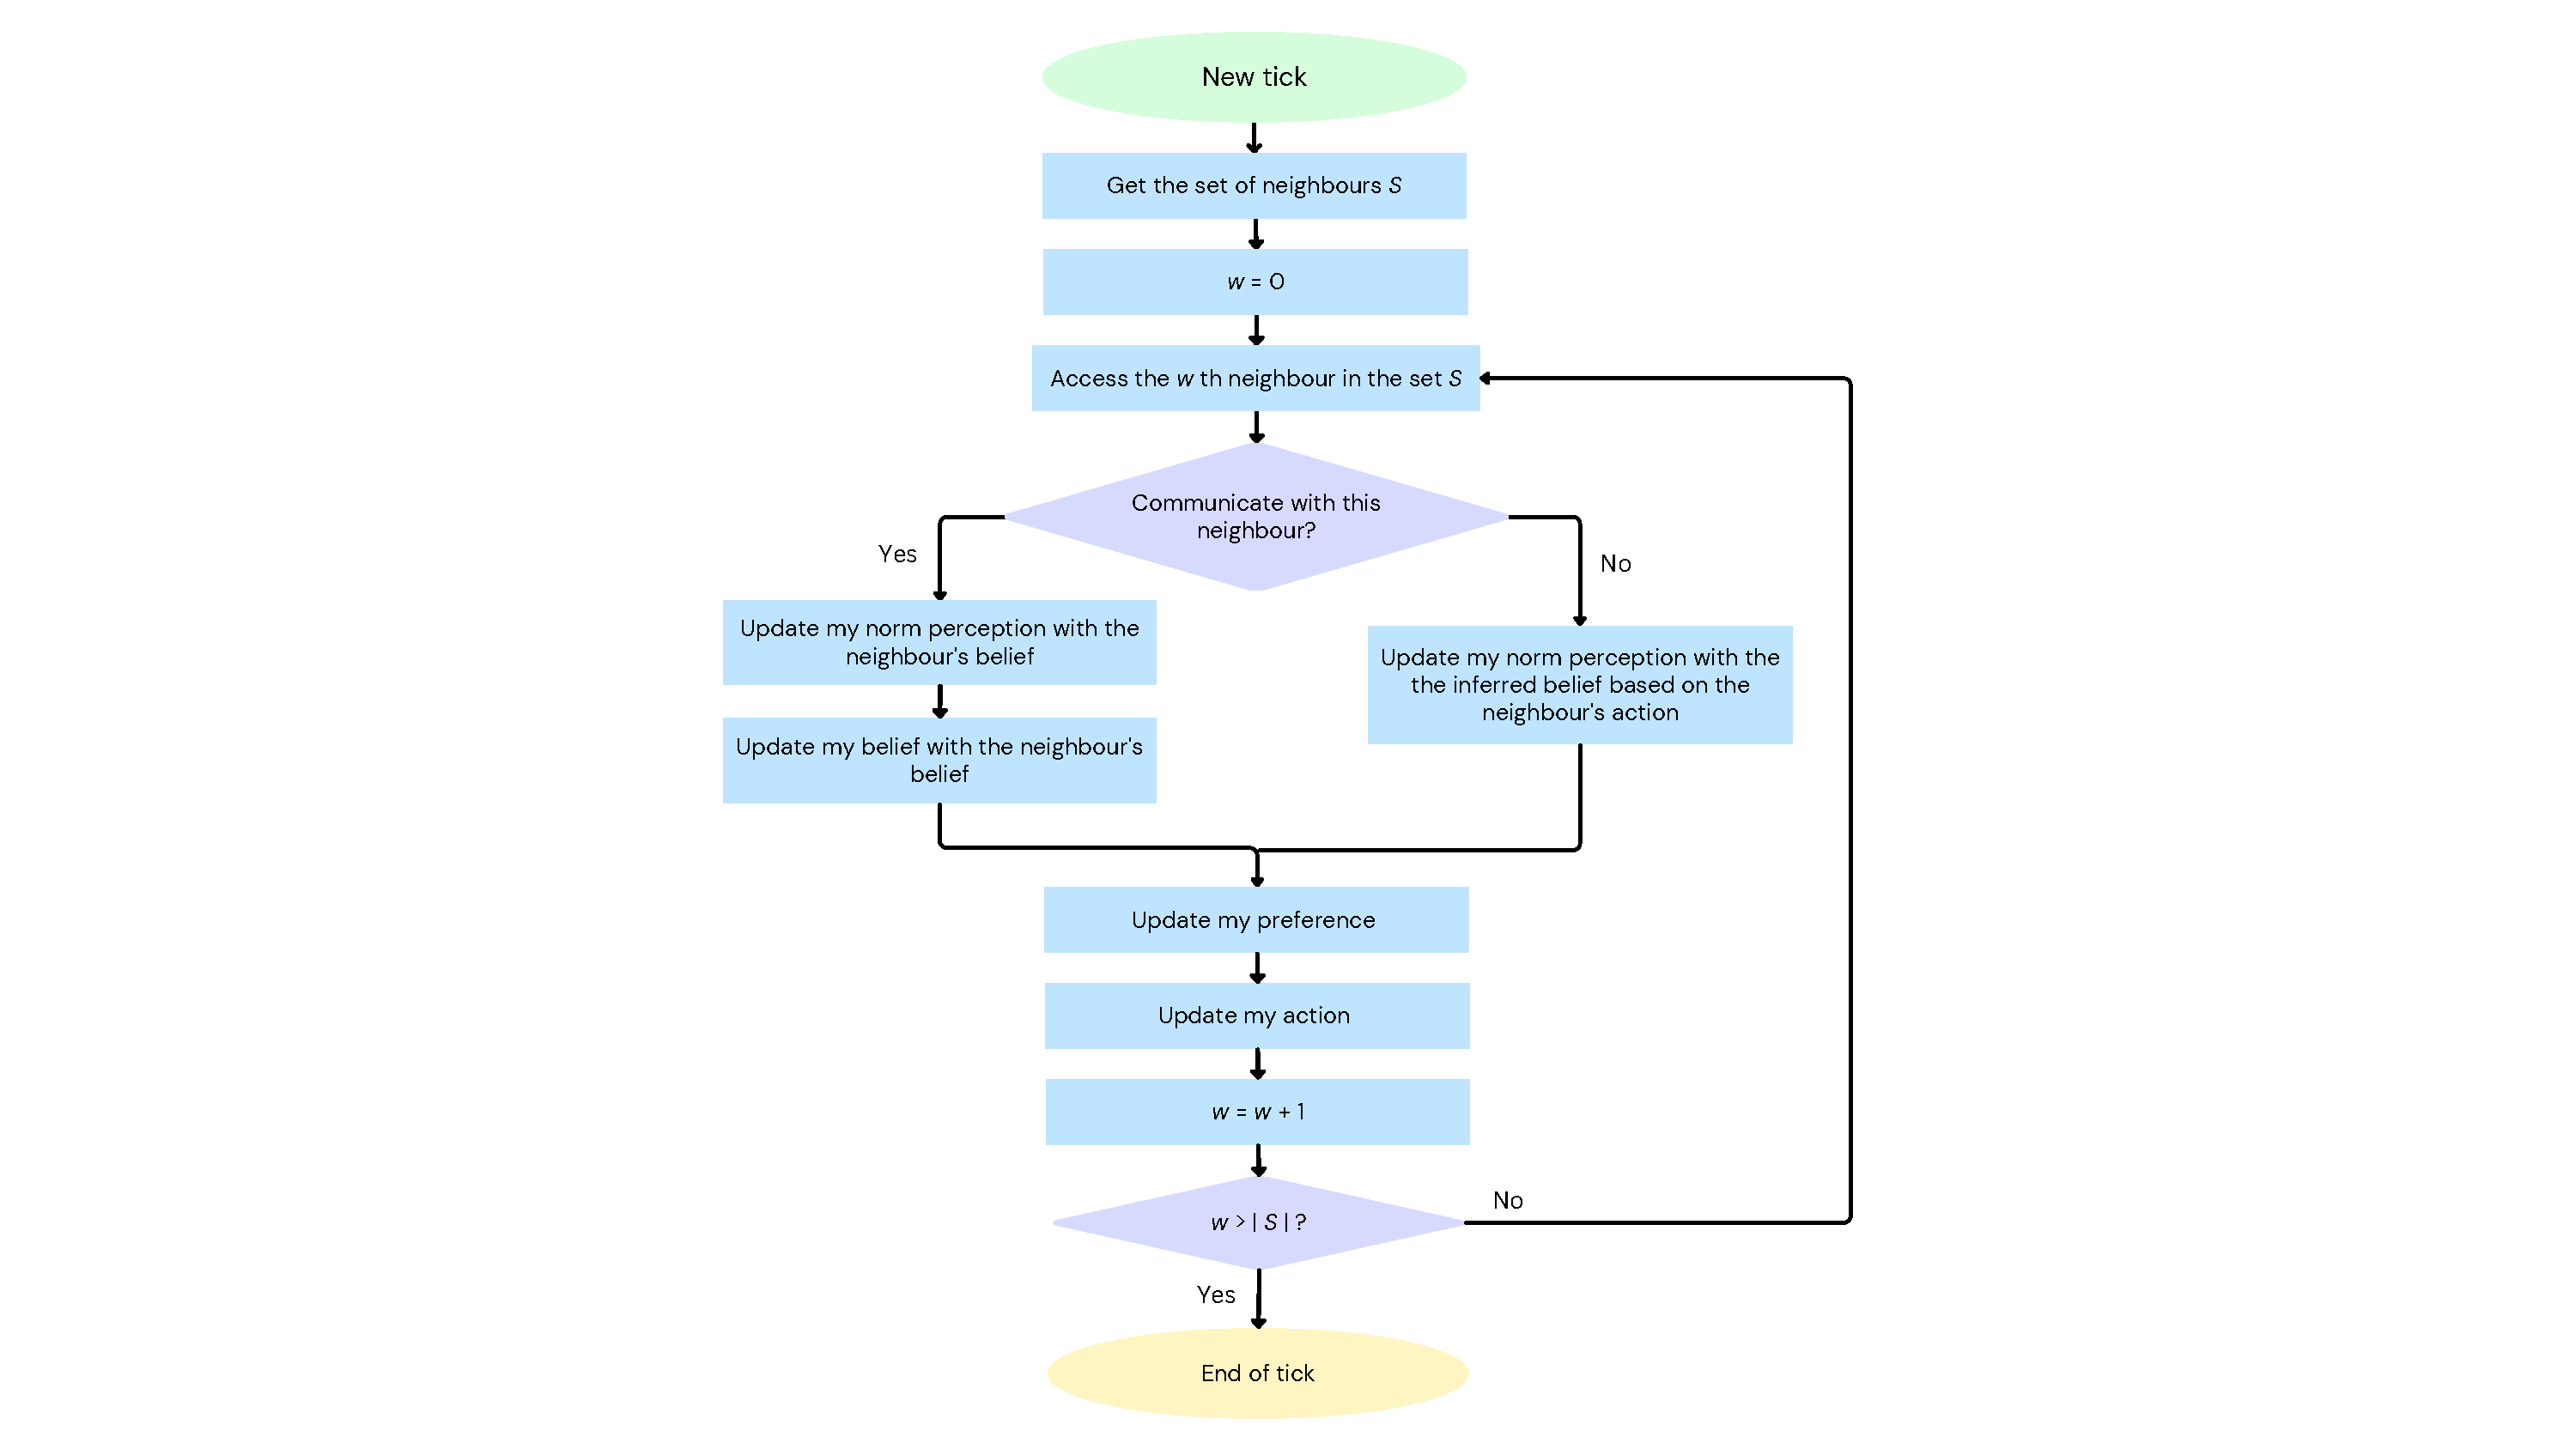
\includegraphics[width=0.7\columnwidth]{./figures/diss_flow_chart.pdf}
  \caption{\textbf{Main updating procedure.} The flow chart shows agents' behaviours at each time step.}
  \label{fig:1}
\end{figure}

Agent \(i\), upon communicating with and accessing the belief of
neighbour \(j\), updating its own belief with bounded confidence. The
bounded confidence model is able to capture the ubiquitous psychological
phenomenon of being more likely to be influenced by people like
ourselves while keeps the computation simple \textbf{(Cialdini \&
Goldstein, 2004)}. Previous research has successfully nested the bounded
confidence model of opinion dynamics in the framework of the CODA model
in the context of a social network, which serves as a foundation for the
current model \textbf{(Zhan et al., 2022)}. Specifically, agent \(i\)
updates its belief based on neighbour \(j\)'s belief using the following
equation:

\begin{equation}
    B_i^{\prime} = \begin{cases}
        B_i, \;\;\;\;\;\;\;\;\;\;\;\;\;\;\;\;\;\;\;\;\;\;\; \text{if} \: |B_i - B_j| > \epsilon_i \\
        B_i + \alpha (B_j - B_i), \; \text{if} \: |B_i - B_j| \le \epsilon_i
    \end{cases}
\end{equation}

where \(\alpha \in (0,0.5]\) is the convergence parameter and
\(\epsilon_i\) is the bounded confidence threshold of the agent \(i\),
which is a value drawn from an exponential distribution with the mean
\(\epsilon_{mean}\) and is a fixed value over time.

Agents update their norm perception \(N_i\) following the Bayesian
inference model \textbf{(Krauß et al.,1999)}. Using Bayes' theorem, we
can update the conditional probability of the agent \(i\)'s norm
perception given evidence using the following equation:

\begin{equation}
\label{eq:2}
f(N_i \mid E_i) = \frac{f(N_i) f(E_i \mid N_i)}{\int f(N_i) f(E_i \mid N_i) dN_i},
\end{equation}

where \(f(N_i)\) denotes the prior probability of norm perception of
agent \(i\), \(E_i\) the evidence (either agent \(j\)'s belief or
inferred belief from its action), and \(f(E_i \mid N_i)\) the
conditional probability of the evidence given \(N_i\). Assuming normal
distributions for both \(f(N_i)\) and \(f(E_i \mid N_i)\), the following
updating rules for the mean and standard deviation of agents' norm
perception can be derived (see the appendices for the derivation):

\begin{equation}
\label{eq:3}
\mu_{N_i}^{\prime} = \lambda \mu_{N_i} + (1 - \lambda) E_i,
\end{equation}

\begin{equation}
\label{eq:4}
\sigma_{N_i}^{\prime2} = \lambda \sigma_{N_i}^2,
\end{equation}

where \(\lambda = \frac{c_i^2}{c_i^2 + \sigma_{N_i}^2}\). The variable
\(c_i\) is agent \(i\)'s confidence in its norm perception (i.e., the
standard deviation of the conditional probability of the evidence,
\(f(E_i \mid N_i)\)), which is drawn from an exponential distribution
with the mean \(c_{mean}\) and is a fixed value over time.

Since agents may or may not communicate with neighbour \(j\), the value
of \(E\) is given by the following equation:

\begin{equation}
  E_i = \begin{cases}
    B_j, \;\;\;\;\;\;\;\;\;\;\;\;\;\;\; \text{if agent} \; i \; \text{communicates with agent} \; j \\
    P(B_j \mid A_j), \;\; \text{if agent} \; i \; \text{doesn't communicate with agent} \; j
  \end{cases}
\end{equation}

\(P(B_j \mid A_j = 1) = 0.9\) and \(P(B_j \mid A_j = 0) = 0.1\) by
stipulation in the simulations reported in the current research.

After updating their belief and norm perception, agents update
preference and action regarding WWOH based on these two values. The
preference is determined by the equation

\begin{equation}
  P_i = r_i B_i + (1 - r_i) N_i,
\end{equation}

where \(r_i\) represents each agent's resistance to social norm, which
is drawn from an exponential distribution with the mean \(r_{mean}\) and
is a fixed value over time. The WWOH action is determined by the
equation:

\begin{equation}
  A_i = \begin{cases}
    0, \;\; \text{if} \; P_i \in [0, 0.5)\\
    1, \;\; \text{if} \; P_i \in [0.5, 1]
  \end{cases}
\end{equation}

\hypertarget{simulations}{%
\subsection{Simulations}\label{simulations}}

\hypertarget{results-2000-2500}{%
\section{Results (2000-2500)}\label{results-2000-2500}}

\hypertarget{discussion-and-conclusion-1000-1500}{%
\section{Discussion and Conclusion
(1000-1500)}\label{discussion-and-conclusion-1000-1500}}

\newpage

\hypertarget{reference}{%
\section*{Reference}\label{reference}}
\addcontentsline{toc}{section}{Reference}

\newpage

\hypertarget{appendices}{%
\section*{Appendices}\label{appendices}}
\addcontentsline{toc}{section}{Appendices}

\hypertarget{the-derivation-of-equation-3-and-4}{%
\subsection*{The Derivation of Equation 3 and
4}\label{the-derivation-of-equation-3-and-4}}
\addcontentsline{toc}{subsection}{The Derivation of Equation 3 and 4}

Since agents' norm perception \(N_i\) is a random variable with a normal
distribution with the mean \(\mu_{N_i}\) and standard deviation
\(\sigma_{N_i}\), we have the probability density function (PDF) of
\(N_i\) as:

\begin{equation*}
f(N_i) \propto \text{exp}(-\frac{(N_i - \mu_{N_i})^2}{2\sigma_{N_i}^2}).
\end{equation*}

The conditional PDF of the evidence given agent \(i\)'s prior norm
perception in Equation \ref{eq:2} is given by

\begin{equation*}
f(E_i \mid N_i) \propto \text{exp}(-\frac{(E_i - N_i)^2}{2c_i^2}).
\end{equation*}

Following the Equation \ref{eq:2}, we have the posterior PDF of agent
\(i\)'s norm perception as

\begin{equation*}
  \begin{aligned}
    f(N_i \mid E_i) &= C \cdot \text{exp}(-\frac{(N_i - \mu_{N_i})^2}{2\sigma_{N_i}^2}) \text{exp}(- \frac{(E_i - N_i)^2}{2c_i^2})\\
      &= C \cdot \text{exp}(-\frac{(N_i - \mu_{N_i})^2}{2\sigma_{N_i}^2} - \frac{(E_i - N_i)^2}{2c_i^2})\\
      &= C \cdot \text{exp}(- \frac{(N_i - \mu_{N_i}^{\prime})^2}{2\sigma_{N_i}^{\prime2}} - \frac{(E_i - \mu_{N_i})^2}{2(\sigma_{N_i}^2 + c_i^2)}),
  \end{aligned}
\end{equation*}

where \(C\) is a normalising constant. Since the second term in the
exponent does not involve the random variable \(N_i\), we can
incorporate it into the constant and rewrite the expression as

\begin{equation*}
  f(N_i \mid E_i) \propto \text{exp}(- \frac{(N_i - \mu_{N_i}^{\prime})^2}{2\sigma_{N_i}^{\prime2}}),
\end{equation*}

where

\begin{equation*}
  \mu_{N_i}^{\prime} = \frac{E_i \sigma_{N_i}^2 + \mu_{N_i} c_i^2}{\sigma_{N_i}^2 + c_i^2} \;\; \text{and} \;\; \sigma_{N_i}^{\prime2} = \frac{\sigma_{N_i}^2 c_i^2}{\sigma_{N_i}^2 + c_i^2}.
\end{equation*}

\end{document}
